
\chapter{ROS与PX4介绍}\label{introduction}

\section{ROS介绍}
本节主要对ROS平台进行介绍,包括ROS核心的消息机制和研究中要用到的gazebo仿真平台。

21世纪开始,随着人工智能研究的发展,催生出了一批智能机器人的研究项目;ROS诞生于2007年斯坦福大学AI实验室Morgan Quigley的STAIR(Standford Artificial Intelligence Robot)项目,其期望构建一个基于移动机器人+机械臂的原型;该项目于2008年受到Willow Garage公司关注,其决定用商业化手段来推进机器人的发展,使机器人平台能够更快地走进人们的日常生活;Willow Garage接手该项目后两年,2010年第一代ROS即ROS1.0发布;2013年,OSRF(Open Source Robotics Foundation)接管了ROS的维护工作和版本的升级工作,随后至2018年间,ROS的Indigo、Kinetic和Melodic版本相继发布。

ROS即Robotics Operating System,是一个针对机器人的开源、元级操作系统,在某些方面,ROS更像是一种机器人框架(robot framework);它提供类似于操作系统的服务,包含底层的驱动程序管理、底层的硬件描述,随后上升到软件程序之间的消息传递、功能包的管理和发布、也提供用于获得、编译、编写和多设备跨计算机运行代码所需的库等。换言之,ROS是由一套通信机制,开发工具,一系列应用功能和一个庞大的生态系统组成的集合,其目标为提高机器人研发中的软件复用率,不断完善他人的工作,进行更好的开发。

\subsection{ROS的消息机制} \label{2.1.1}

% ROS松耦合分布式通信+引出节点
ROS提供了一套松耦合分布式通信机制,这种分布式处理框架(又名Nodes),是以多个节点及节点之间的通信组成的。其中,节点(Node)和节点管理器(ROS Master)是ROS的核心概念,若干个节点在节点管理器下构建起来,共同实现特定的功能。

% 介绍节点的作用
每一个节点是一个独立的执行单元,由可执行文件构成,在程序中需要声明节点的名称;节点的名称必须唯一,否则ROS会舍弃掉时间节点靠前的节点;节点执行具体的任务进程,比如单目的ORB-SLAM2中,其节点为Mono,SLAM的任务仅靠一个节点完成。

% 介绍节点管理器
节点管理器是节点的控制中心,其作用是辅助节点的查找,帮助节点之间建立通信连接;还能提供节点的命名和注册等服务,以及提供了能够存储全局变量的配置的参数服务器。

\begin{figure}[!ht]
\centering
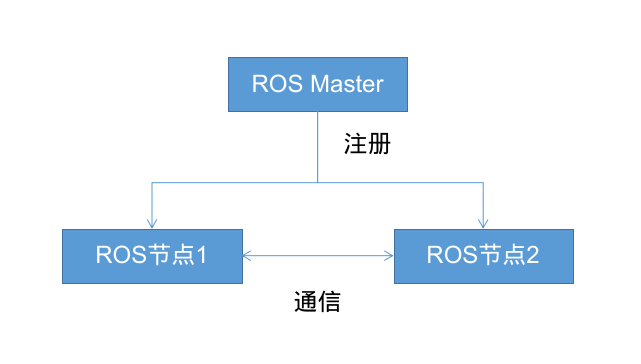
\includegraphics[width=0.6\textwidth]{ros_node.png}
\caption{ROS中的节点及通信} 
\label{fig2}
\end{figure}

% 介绍节点的通信
如图\ref{fig2}所示,节点在经过节点管理器注册后,可以建立节点之间的通信;常用的节点之间通信方式有两种,为话题(Topic)通信和服务(Service)通信:
\begin{enumerate}
	\item 话题通信是异步通信机制,数据为单向传输;数据的流向为发布者(Publisher)到订阅者(Subscriber);完成话题通信需要定义一个话题(Topic)及其消息(Message)的内容,之后通过发布者(Publisher)发布该话题,并且订阅者(Subscriber)订阅该话题的操作,完成数据的传输,消息的数据结构由.msg文件定义;话题通信可以完成多对多的信息传递。
	\item 
	服务的通信机制则为同步,数据为双向传输;数据的流向为客户端(Client)与服务器(Server)之间的交互;完成服务的通信需要客户端向服务器发送请求,服务器完成任务处理后,向客户端返回应答数据,表示请求和应答的数据结构定义在.srv文件中;服务通信一般用于逻辑判断,比如询问一项任务是否执行完毕,是一对多的节点处理关系。
\end{enumerate}

% 介绍Topic的编程
发布和订阅话题的方法,发布者和订阅者类似,以发布者为例:先实例化一个发布者对象,定义发布的话题名称、数据类型和队列长度,最后对消息进行定义并发送,简单的逻辑代码如下:
\begin{lstlisting}[language={C++}]
ros::NodeHandle n;  // define ros node handle
// define a publisher
ros::Publisher pub = n.advertise<'message type'>
	("topic name", `queue length`);
// publish message
pub.publish(message);
\end{lstlisting}

需要注意的是,订阅者则需要声明并定义一个回调函数,在实例化Subscriber的对象后,通过ROS的spin()函数,循环等待回调函数获得话题消息。

% 介绍Service的编程
客户端-服务器模型下的服务通信,则比话题的发布和订阅复杂;客户端的编程实现中,需要设置阻塞函数,其作用是直到发现对应的服务时才向下进行,否则程序被截止在该位置;如果对应的服务被发现,阻塞函数通过,之后创建客户端并且进行数据的设置,完成服务调用的请求,其代码实现如下:
\begin{lstlisting}[language={C++}]
// wait for right service
ros::service::waitForService("service name");
// create a client, connecting to service
ros::ServiceClient client = n.serviceClient
	<'data type'>("service name");
// call service
client.call(srv);
\end{lstlisting}

服务器的实现与订阅者类似,需要一个回调函数,如果收到了客户端发来的请求,则会触发回调函数,程序向下进行,否则将循环等待回调函数收到客户端发来的请求。

% 介绍参数服务器
除此之外,ROS中还有参数(Parameter)或参数服务器的概念,其作用类似全局共享字典,节点可以进行访问,适合存储一些和系统配置相关的静态非二进制的参数,以供节点读取。


\subsection{gazebo仿真} \label{2.1.2}
gazebo是ROS自带的仿真软件,



\section{PX4 AutoPilot}
本文将飞行摇杆(Joystick)数据读取作为四旋翼飞控模型的输入,Joystick数据的数据主要是四旋翼的姿态角(滚转角,偏航角,俯仰角)和四旋翼的推力。因此,本文通过C++编程,实现飞行摇杆数据的输入。由如下代码所示:

\begin{lstlisting}[language={[ANSI]C++}]
class HAL_JoyStick: public ZY::Thread {
public:
    HAL_JoyStick(){
        m_devID = -1;
    }
    HAL_JoyStick(int dev) {
        m_devID=dev;
    }
    virtual ~HAL_JoyStick() {}
    int open(int devID);
    void run();
    int close(void);
    int read(JS_Val *jsv)
    {
        data_mutex.lock();
        *jsv= m_JSVal;
        m_JSVal.dataUpdated = 0;
        data_mutex.unlock();
        return 0;
    }
public:
    int         m_devType;
    int         m_devID;
    int         m_devFD;
    char        number_of_axes;
    char        number_of_btns;
protected:
    ZY::Mutex   data_mutex;
    JS_Val      m_JSVal;
}
\end{lstlisting}

\subsection{FailSafe机制} \label{2.2.1}
\subsection{EKF与飞行模式} \label{2.2.2}
\subsection{联合MAVROS的Offboard模式} \label{2.2.3}



